\chapter{Related work}
\label{chap:rel_work}
%TODO when done, fix this
In this chapter we discuss the relevant literature and state of the art for this thesis, the literature is grouped in x groups. In \autoref{section:routing_rel_work} the routing algorithms for transport are discussed. Next, we discuss the data models used in public transport, either by law or popularity (\autoref{section:data_model_rel_work}). Further, we look at developed ontologies for transportation in \autoref{section:ontologies_rel_work}.

\section{Transport Routing Algorithms }\label{section:routing_rel_work}
% include timeline image

\input{tikz/tikz_timeline}

In this section, we discuss the state of the art and history of public transport planning. Therefore a small timeline (\autoref{fig:timeline}) was constructed to visualize some important milestones explained below. As seen in the timeline most advances were made after 2009.

\subsection{Dijkstra}
% add some dijkstra algo workings, easy
The milestones between 1956 and 2008 did not apply to PT routing but focused on normal road networks. Among these milestones was the Dijkstra algorithm published in 1958. This was the first big improvement but had a time complexity of $O(n^2)$. An improved version was proposed almost 30 years later in 1987. It has a complexity of $O(n*\log(n))$ and is the version of the Dijkstra algorithm learnt at schools.% It works by initializing every node to $\infty$ except the source node, which is initialized to $0$. Then every edge of the source node is visited. 
\subsection{Dimacs challenge}
No big improvements for route planners were made until 2005. The road network of the US was published as part of the 9th Dimacs challenge \cite{noauthor_9th_2017}. A big deal for researchers, now they had a big dataset to test on. A lot of speed-up techniques were devised for the Dijkstra algorithms, mainly pruning techniques. But this was still inapplicable to \glsxtrshort{pt}.

\subsection{Car or Public Transport: Two Worlds}
In 2009 a paper, Car or Public Transport: Two Worlds \cite{bast_car_2009}, stated "There are two kinds of people: those who travel by car, and those who use public transport.". They argued that the worlds were different although both problems could be represented as a directed graph. For PT we require dealing with timetable schedules beside this spatial information.

The article covers 5 big "tricks of the trade" for fast routing on transportation: Bidirectional search, exploiting hierarchy, graph contraction, goal direction and distance tables. It explains why the trick works on road networks but falls short on \glsxtrshort{pt}.

\subsubsection{Bidirectional search}
A simple approach to improve Dijkstra is to search from the source node but simultaneously do a backward search from the target node. This reduces the search space by half and can be easily done for road networks since both nodes associated with the station are known. The idea by itself is not very effective but is key to implementing other speedup techniques.

For \glsxtrshort{pt} this idea adds a lot of complexity since in a time-expanded graph we know the target station but not the target node. A solution is to do a backward set of all nodes associated with the end station.
\subsubsection{Exploiting hierarchy}
Roads have different levels of importance, think of motorways, national roads and small roads. The simple routing heuristic exploits this hierarchy. When we are within a certain distance of the target and source node, we take all roads into account. In the other case, we use only high-level roads, reducing the total explored nodes. This comes with some loss of exactness.

However, in large municipal areas, this technique can be even slower, because the hierarchy is absent. The tram, metro and bus are equally important. Only when travelling long distances between cities, does a hierarchy begin to appear. 
\subsubsection{Graph contraction}
\subsubsection{Goal direction}
\subsubsection{Distance tables}


This overview article marked the beginning of new PT route planners that were in the same ballpark as road networks in terms of query speed. 
\subsection{Transfer patterns}
Transfer patterns are considered the first algorithm for PT that solves queries in an order of a few milliseconds and on a transport network with a poor structure. 

Transfer patterns describe a method using a journey planning algorithm to pre-calculate all the unique journeys for the entire graph \cite{bast_fast_2010} %wrong explanation of transfer graphs TODO FIX
. This means when a real-time query comes in we can look up the schedule that matches that journey. In this case, the server can give fast query responses, but the pre-calculations can cause a computational burden. For example, the authors used a cluster of Opteron and Xeon-based 64-bit servers for their CPP implementation. Although the exact number of compute nodes is not mentioned in the paper \cite{bast_fast_2010}. 


% TODO uitleggen transfer paterns
A simple algorithm for transfer patterns illustrates the key ideas and consists of 3 parts, but has quadratic precomputation complexity.
\subsubsection{Graph}
The algorithm works on a time-expanded graph with three kinds of nodes: a departure node, an arrival node and a transfer node. Each node carries the time and the station it belongs to. An elementary connection can be formed like in \autoref{fig:transferel}.
\begin{figure}[H]
\begin{minipage}{.45\textwidth}

\centering
\resizebox{0.5\linewidth}{!}{%
    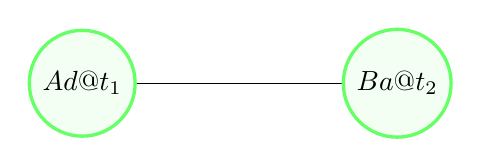
\begin{tikzpicture}[
roundnode/.style={circle, draw=green!60, fill=green!5, very thick, minimum size=8mm},
]
    
    \draw (0,0) -- (4,0);
    
    \draw (4,0) node[align=center,roundnode] {$Ba@t_2$};

    \draw (0,0) node[align=center,roundnode] {$Ad@t_1$};
    
    \end{tikzpicture}
%
}%
    \caption{An elementary connection betweens stations A and B, d stands for departure and a for arrival, $@t_i$ denotes the time the vehicle departs, arrives are waits (transfer)}
    \label{fig:transferel}

\end{minipage}\hspace{.1\textwidth}
\begin{minipage}{.45\textwidth}
\centering
\resizebox{0.5\linewidth}{!}{%
    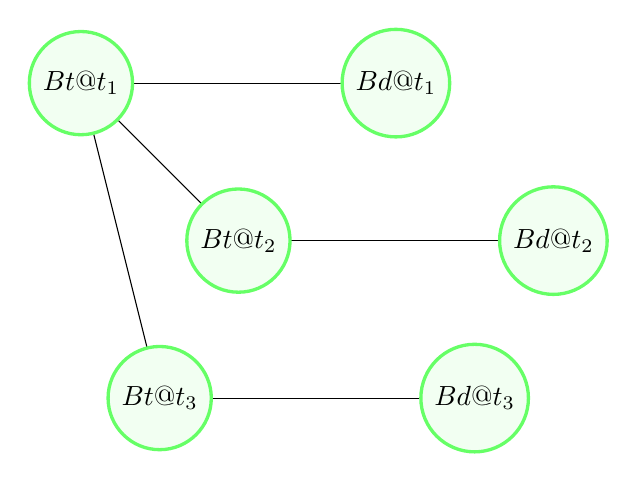
\begin{tikzpicture}[
roundnode/.style={circle, draw=green!60, fill=green!5, very thick, minimum size=8mm},
]
    
    \draw (0,0) -- (4,0);
    \draw (0,0) -- (2,-2);
    \draw (0,0) -- (1,-4);
    \draw (1,-4) -- (5,-4);
    \draw (2,-2) -- (6,-2);
    
    \draw (0,0) node[align=center,roundnode] {$Bt@t_1$};

    \draw (4,0) node[align=center,roundnode] {$Bd@t_1$};


    
    \draw (2,-2) node[align=center,roundnode] {$Bt@t_2$};

    \draw (6,-2) node[align=center,roundnode] {$Bd@t_2$};

    \draw (1,-4) node[align=center,roundnode] {$Bt@t_3$};

    \draw (5,-4) node[align=center,roundnode] {$Bd@t_3$};
    \end{tikzpicture}
%
}%
    \caption{An transfer, with an waiting chain}
    \label{fig:transferpatterntransfer}

\end{minipage}
\end{figure}
\subsubsection{Fast direct-connections queries}
This part is only for direct connections, meaning a maximal path in the graph without transfer nodes.

\begin{enumerate}
    \item Precompute all maximal paths in the graph without transfer nodes. Group them in lines that share the same sequence of stations. This creates an ordered timetable for a particular line.
    \item Precompute for each station,  the sorted list of lines in which the station occurs and its position(s) on the line. This creates a lookup table, which can be used to find timetables of lines stations share.
    \item To answer a direct connection query use the precomputed sorted list of the departure and arrival stations. See if they share a line with the departure station, which has a lower position than the arrival station. Using the timetables of the found lines, determine the earliest arrival time.
\end{enumerate}
\subsubsection{Transfer patterns precomputation}
\subsubsection{Query graph construction and evaluation}
\subsubsection{scalable transfer patterns}
% IDEA, HYDRIDE? 
\subsection{\glsfmtfull{csa}}
\subsection{\glsfmtfull{raptor}}
RAPTOR is a graph-based algorithm which solves queries in rounds. Round K computes the fastest way of getting to every stop with at most k - 1 transfers or k trips.

\begin{enumerate}
    \item Each node gets a multilabel. $(\tau_0,...,\tau_k)$ with $\tau_i$ representing the earliest arrival time in $i$ trips. We init all arrival times in each label with $\infty$. Except for the departing node, where $\tau_0$ is set to the depart time of our search criteria.
    \item For each round $k$ our goal is to compute $\tau_k$. This happens in three stages:\begin{enumerate}
        \item Set the earliest arrival time k ($\tau_k$) to that of iets predescor ($\tau_{k-1}$). This is an upper bound since we are not interested in slower stop times than the previous round.
        \item We iterate over the routes. We calculate for each stop $p$ on the route $r$, the earliest trip we can take. This does not always exist. We search stops along the route $r$ that has the earliest trip $t$. This means we can hop on the route $r'$ in $p$. For subsequent stops in $r'$, we can update $\tau_k$ according to the found trip $t$.
        \item Finally, footpaths are considered. We check if $\tau_k$ can be improved by using a footpath between two stops. 
    \end{enumerate}
\end{enumerate}


\begin{figure}[H]
\centering
\resizebox{\textwidth}{!}{%
    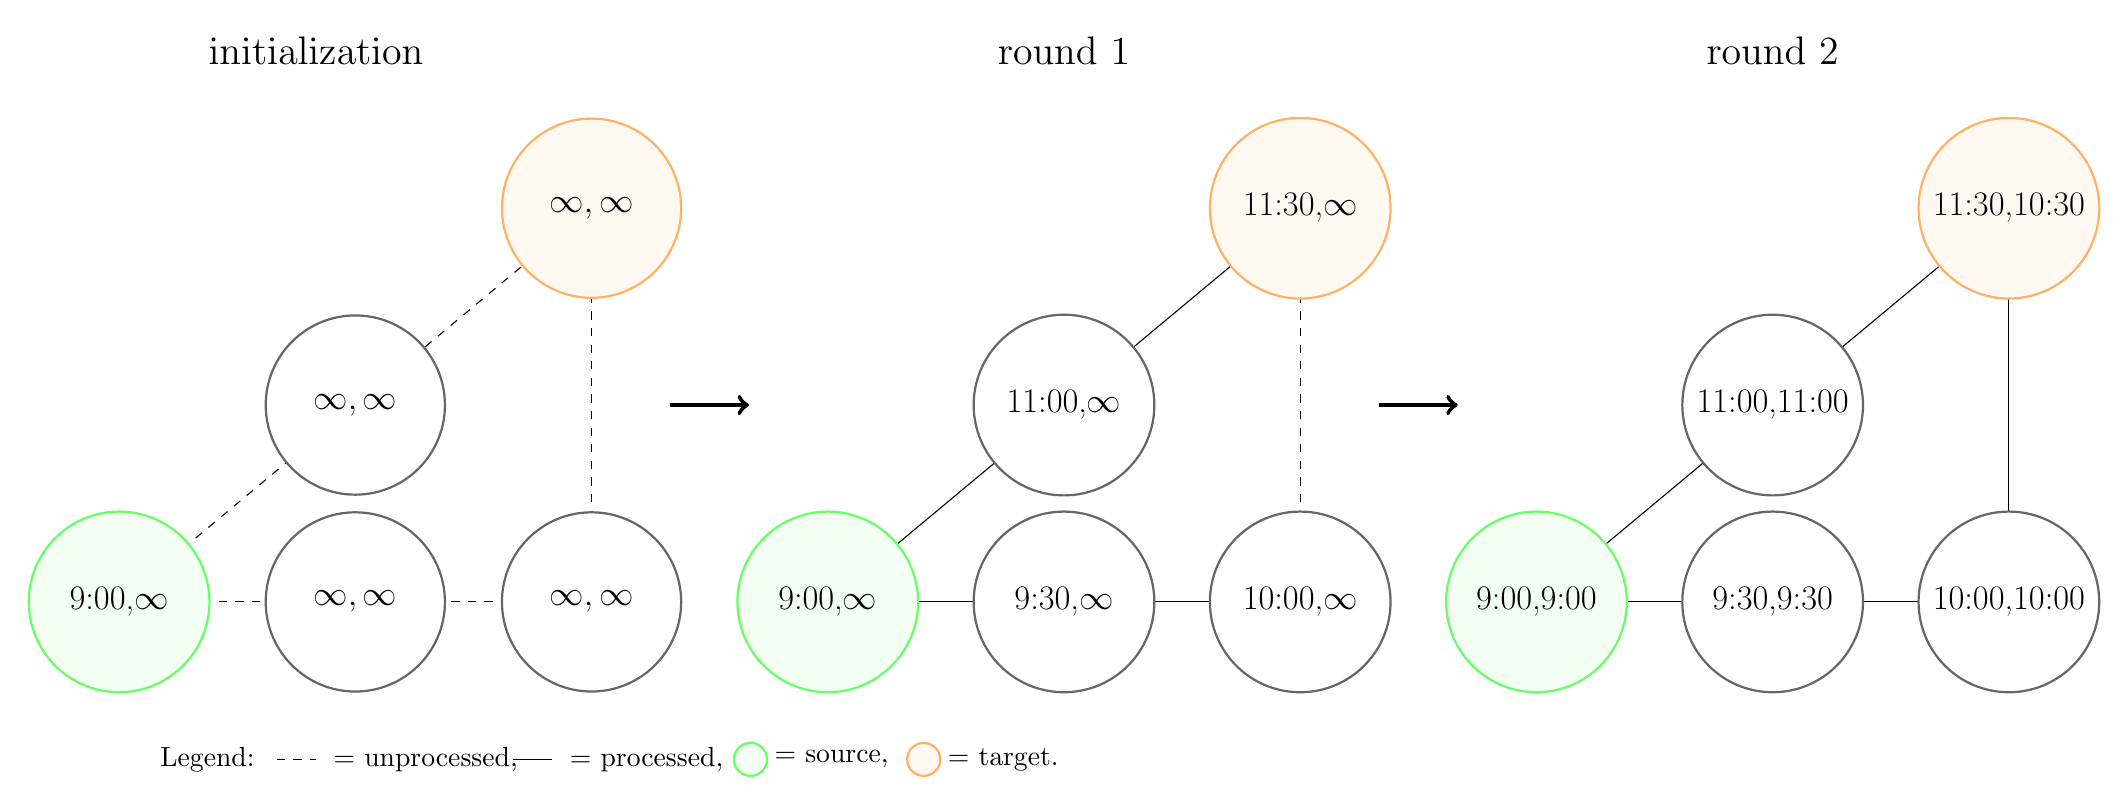
\begin{tikzpicture}[
roundnode/.style={circle, thick, minimum size=7mm, text width=3.5cm,align = center,scale=0.6,font=\huge},
green/.style={draw=green!60, fill=green!5},
orange/.style={draw=orange!60, fill=orange!5},
white/.style={draw=black!60, fill=white},
]
    \draw (0.4,-2) node[right=0] {Legend:};
    \draw [dashed](2,-2) -- (2.5,-2);
    \draw (2.6,-2) node[right=0] {= unprocessed,};
    \draw [](5,-2) -- (5.5,-2);
    \draw (5.6,-2) node[right=0] {= processed,};
    \draw (7.8,-2) node[roundnode,text width=0.4cm,green,right=0] {};
    \draw (8.2,-2) node[right=0] {= source,};
    \draw (10,-2) node[roundnode,text width=0.4cm,orange,right=0] {};
    \draw (10.4,-2) node[right=0] {= target.};
    
    \draw [dashed](0,0) -- (6,0);
    \draw [](9,0) -- (15,0);
    \draw [](18,0) -- (24,0);
    

    \draw [dashed](6,0) -- (6,5);
    \draw [dashed](15,0) -- (15,5);
    \draw [](24,0) -- (24,5);
    

    \draw [dashed](0,0) -- (6,5);
    \draw [](9,0) -- (15,5);
    \draw [](18,0) -- (24,5);
    
    \draw[->, ultra thick] (7,2.5) -- (8,2.5);
    \draw[->, ultra thick] (16,2.5) -- (17,2.5);
    
    \draw (0,0) node[roundnode,green] {9:00,$\infty$};
    \draw (3,0) node[roundnode,white] {$\infty,\infty$};
    \draw (6,0) node[roundnode,white] {$\infty,\infty$};
    \draw (3,2.5) node[roundnode,white] {$\infty,\infty$};
    \draw (6,5) node[roundnode,orange] {$\infty,\infty$};

    
    \draw (9,0) node[roundnode,green] {9:00,$\infty$};
    \draw (12,0) node[roundnode,white] {9:30,$\infty$};
    \draw (15,0) node[roundnode,white] {10:00,$\infty$};
    \draw (12,2.5) node[roundnode,white] {11:00,$\infty$};
    \draw (15,5) node[roundnode,orange] {11:30,$\infty$};

    
    \draw (18,0) node[roundnode,green] {9:00,9:00};
    \draw (21,0) node[roundnode,white] {9:30,9:30};
    \draw (24,0) node[roundnode,white] {10:00,10:00};
    \draw (21,2.5) node[roundnode,white] {11:00,11:00};
    \draw (24,5) node[roundnode,orange] {11:30,10:30};

    \draw (2.5,7) node[font=\Large] {initialization};
    \draw (12,7) node[font=\Large] {round 1};
    \draw (21,7) node[font=\Large] {round 2};
    \end{tikzpicture}
%
}%
    \caption{A small example using raptor, two rounds are show}
    \label{fig:raptor_example}
\end{figure}

\subsubsection{Hyper partitioning}
Hyper partitioning is a preprocessing-based acceleration technique for computing bi-criteria Pareto-optimal journeys in public transit networks, based on the well-known RAPTOR algorithm \cite{delling_round-based_2015}.
\subsubsection{unrestricted footprints}
\section{Data Models For public transport}\label{section:data_model_rel_work}
\subsection{What is a data model }
% TODO CHECK AND REWRITE 
% FROM https://cedar.princeton.edu/understanding-data/what-data-model
A data model organizes data elements and standardizes how the data elements relate to one another. Since data elements document real-life people, places and things and the events between them, the data model represents reality. For example, a house has many windows or a cat has two eyes.

Data models are often used as an aid to communication between the business people defining the requirements for a computer system and the technical people defining the design in response to those requirements. They are used to show the data needed and created by business processes.
 
A data model explicitly determines the structure of data. Data models are specified in a data modelling notation, which is often graphical in form.]
A data model can be sometimes referred to as a data structure, especially in the context of programming languages. Data models are often complemented by function models.
\subsection{\glsfmtfull{gtfs}}
\glsfmtfull{gtfs} defines a common format for public transportation schedules and associated geographic information. "feeds" let public transit agencies publish their transit data. The developer can then write applications.
\subsubsection{\glsfmtshort{gtfs} feed}
A feed is a zip file that contains CSV files, but typically uses the .txt extension. Some important files include stops.txt, routes.txt and trips.txt.


\subsection{\glsfmtfull{netex}}
The NeTEx defines a standard for exchanging public transport passenger information data in XML format. The functional
scope of NeTEx is divided into three parts, each covering a functional subset of the CEN Transmodel conceptual
model for Public Transport Information, [T1], [T2], [T3].
Part 1 [N1]] describes the fixed Network (stops, routes, lines, etc.); Part 2 [N2] is mainly focused on Timetables and
Part 3 [N3] covers Fare data (and is the main subject of this paper). All three parts use the same framework of reusable
components, versioning mechanism, validity conditions, and support to allow the unique identification of data elements
in a global context, etc., defined in Part 1. NeTEx also includes container elements called “VERSION FRAMES”
to group data into coherent sets for efficient exchange.
NeTEx deliverables comprise (i) a CEN Specification document (in three parts), (ii) a data model in the standard UML
modelling language [U1] and (iii) an accompanying XML schema providing a formal electronic description that can
be used by data processing software.

Data in NeTEx format is encoded as XML documents that must conform exactly to the schema – standard XML validator tools can check conformance automatically. The schema can also be used to create bindings for different
programming languages, automating part of the implementation process for creating software that supports NeTEx
formats. 
\subsubsection{NETEX profiles}
\subsection{Transmodel}
\section{Semantic Web and the role of Ontologies}\label{section:ontologies_rel_work}
\subsection{Semantic Web}
The semantic web can be seen as an extension of the current web and is a vision of Tim Berners-Lee, where web documents not only describe how to render data visually. The data is also annotated with terms to express how it should be interpreted. So web documents also capture the meaning of the information.
\subsection{Resource Description Framework}
\subsection{JSON-LD}
%\subsection{RML}

\subsection{Ontologies}
The best definition of an ontology states: "An ontology is an explicit specification of a conceptualization"\cite{gruber_translation_1993}. Many ontologies exist, from basic to formal ontologies specified in highly expressive logic. In this thesis, we mainly use formal ontologies.

These ontologies play an essential role in the semantic web. 

A small study was conducted to find an ontology that best suited our needs. Many of the studied ontologies for transport are focused on specific use cases, for example, urban freight \cite{bouhana_ontology-based_2015}. They do not have a broad domain. 
\subsection{x}
A relatively old ontology designed to use with a user planning tool based on journey patterns \cite{5507372} was found and could support RAPTOR. Interestingly, they implemented a mobile application to plan tourist bus routes, but it relied on server-side queries. Other downsides are that there is no multi-modal support (only transport by bus) and no multi-operator support. The ontology was not directly available from the authors.

Using the survey of transportation ontologies \cite{katsumi_ontologies_2018}, we only identify three ontologies that support journey patterns. Two are focused on city logistics and urban systems, a different domain. The last ontology (Transportation ontology for content personalization) applies to PT, but the ontology is not directly available.

\subsection{Transmodel ontology}
European directives require every PT agent to be compatible with Transmodel, so an ontology aligned with Transmodel is interesting. Further, the Transmodel ontology supports journey patterns. However, the ontology could be too broad, which leads to several potential problems. For example, it can make it hard to find relevant information, as the ontology may contain too many concepts and relationships that are not relevant. Furthermore, as the ontology may not be compatible with other ontologies used in those sources, integration from different sources can also be challenging.

\subsection{OSLO Mobiliteit: Dienstregeling en Planning}
The last ontology we looked at is the "OSLO Mobiliteit - Dienstregeling en Planning" \cite{noauthor_oslo_2023} ontology. The ontology is developed by Open Standaarden voor Linkende Organisaties (OSLO), a department of Data Flanders. It has been based on the EPIP profile of NETEX. NETEX is based directly on  Transmodel, so the ontology has some similarities with the Transmodel ontology but is less broad than the Transmodel ontology.

\begin{landscape}
\begin{table}[]
\centering
\begin{tabular}{|l|l|l|l|l|l|l|}
\hline
\textbf{Ontology} &
  \textbf{\begin{tabular}[c]{@{}l@{}}Journey\\ patterns?\end{tabular}} &
  \textbf{\begin{tabular}[c]{@{}l@{}}Multi-\\ modal?\end{tabular}} &
  \textbf{\begin{tabular}[c]{@{}l@{}}Multi-\\ operator?\end{tabular}} &
  \textbf{\begin{tabular}[c]{@{}l@{}}Designed for use\\  with routeplanners\end{tabular}} &
  \textbf{\begin{tabular}[c]{@{}l@{}}directly available\\  for reuse?\end{tabular}} &
  \textbf{DOI} \\ \hline
\begin{tabular}[c]{@{}l@{}}Intoducing the public transport\\ domain to the web of data\end{tabular} &
  yes &
  yes &
  yes &
  yes &
  no &
  10.1007/978-3-319-11746-1\_38a \\ \hline
iCity Ontology &
  yes &
  no &
  no &
  no, urban systems &
  yes, GitHub &
  w3id.org/icity/iCityOntology\_v1\_Report.pdf \\ \hline
Genclon &
  yes &
  no &
  no &
  no, city logistics &
  no &
  10.1016/j.eswa.2012.03.068 \\ \hline
\begin{tabular}[c]{@{}l@{}}Transportation ontology\\ for content personalization\end{tabular} &
  yes &
  yes &
  yes &
  yes &
  no &
  10.1016/j.eswa.2012.12.028 \\ \hline
Transmodel ontology &
  yes &
  yes &
  yes &
  yes &
  yes, GitHub &
  10.3233/SW-210451 \\ \hline
OSLO Ontology &
  yes &
  yes &
  yes &
  yes &
  yes &
  / \\ \hline
\end{tabular}
\caption{}
\label{tab:my-table}
\end{table}
\end{landscape}